% ---------------------------------------------------------------
% OUP Bioinformatics-style report — fully self-contained
% Compiles on Overleaf or any standard LaTeX install (no extra .cls needed)
% ---------------------------------------------------------------
\documentclass[10pt,twocolumn]{article}

\usepackage[top=2cm,bottom=2cm,left=1.8cm,right=1.8cm,columnsep=0.6cm]{geometry}
\usepackage{graphicx}
\usepackage{booktabs}
\usepackage{amsmath}
\usepackage[numbers,sort&compress]{natbib}
\usepackage[colorlinks=true,linkcolor=blue,citecolor=blue,urlcolor=blue]{hyperref}
\usepackage[T1]{fontenc}
\usepackage{parskip}
\usepackage{titlesec}
\usepackage{fancyhdr}
\usepackage{xcolor}
\usepackage{caption}
\usepackage{times}
\usepackage{courier}

% ---- Section formatting (OUP style) ----------------------------
\titleformat{\section}{\normalfont\bfseries\large}{\thesection.}{0.5em}{}
\titleformat{\subsection}{\normalfont\bfseries\normalsize}{\thesubsection}{0.5em}{}
\titleformat{\subsubsection}[runin]{\normalfont\bfseries\small}{}{0pt}{}[.\enspace]
\titlespacing*{\section}{0pt}{10pt}{4pt}
\titlespacing*{\subsection}{0pt}{8pt}{2pt}

% ---- Caption formatting ----------------------------------------
\captionsetup{font=small,labelfont=bf,labelsep=period}

% ---- Header / footer -------------------------------------------
\pagestyle{fancy}
\fancyhf{}
\fancyhead[L]{\small\textit{Bioinformatics}, 2026, 1--5}
\fancyhead[R]{\small Pathak}
\fancyfoot[C]{\small\thepage}
\renewcommand{\headrulewidth}{0.4pt}

% ----------------------------------------------------------------
\begin{document}

% ---- Title block -----------------------------------------------
\twocolumn[{%
\begin{@twocolumnfalse}

\vspace*{6pt}
{\noindent\small Original Paper \hfill \textit{Bioinformatics} \textbf{00}(00), 2026, 1--5
\par\vspace{4pt}\hrule\vspace{10pt}}

{\noindent\LARGE\bfseries
  Benchmarking Regression-Based Cell Type Deconvolution\\[4pt]
  Methods for Bulk RNA-seq Data
\par}

\vspace{8pt}

{\noindent\normalsize
  \textbf{Vignesh Pathak}\\[2pt]
  Department of Computer Science, University of Illinois Chicago,
  851 S Morgan St, Chicago, IL 60607, USA\\[2pt]
  \textit{Corresponding author.}
\par}

\vspace{8pt}

% ---- Structured abstract (OUP Bioinformatics format) -----------
\begin{abstract}
\noindent\textbf{Motivation:}
Determining cell type composition from bulk RNA-seq data is fundamental
to computational biology, with direct applications in cancer immunology and
disease characterisation. Reference-based deconvolution frames this as a
regression problem: given an observed bulk expression vector and a reference
signature matrix, recover non-negative cell type proportions. Widely-used
tools such as CIBERSORTx and MuSiC embed specific regression engines as
black boxes, yet it remains unclear whether the regression algorithm
materially affects accuracy or whether upstream factors such as signature
matrix quality and gene selection dominate performance.

\medskip\noindent\textbf{Results:}
We benchmarked three algorithms---Non-Negative Least Squares (NNLS), Support
Vector Regression (SVR), and Robust Regression via Huber loss---on synthetic
pseudo-bulk mixtures from 8 immune cell types using GEO dataset GSE107011.
All three methods achieve strong accuracy (Pearson $r>0.94$) with differences
of $\Delta r<0.003$ across methods. NNLS matches or exceeds competing methods
on every accuracy metric, exhibits the greatest noise stability, and is
approximately 3\,000$\times$ faster than SVR. Marker gene selection strategy
and cell type transcriptomic distinctness are larger determinants of
deconvolution quality than the choice of regression algorithm.

\medskip\noindent\textbf{Availability and Implementation:}
All code is implemented in Python 3.10 using scipy, scikit-learn, and
statsmodels and is available at
\href{https://github.com/VighneshDev1411/deconv-benchmark}{\textcolor{blue}{github.com/VighneshDev1411/deconv-benchmark}}.

\medskip\noindent\textbf{Contact:}
\href{mailto:vpath6@uic.edu}{vpath6@uic.edu}
\end{abstract}

\vspace{6pt}\hrule\vspace{12pt}
\end{@twocolumnfalse}
}]

% ================================================================
\section{Introduction}

Bulk RNA-seq measures aggregate gene expression from tissue samples
containing thousands of cells of heterogeneous types. The resulting profile
is a weighted mixture of constituent cell type expression programmes, where
weights correspond to cell type proportions. Accurate recovery of these
proportions is essential for characterising the tumour microenvironment,
profiling immune responses, and identifying cellular correlates of disease
progression \citep{wang2019}.

Reference-based deconvolution solves for proportions by fitting a mixture
model: given observed bulk expression $\mathbf{b}$ and reference signature
matrix $S$ (columns = mean expression per cell type), recover non-negative
coefficients $\mathbf{c}$ such that $S\mathbf{c}\approx\mathbf{b}$. Tools
such as CIBERSORTx \citep{newman2019}, MuSiC \citep{wang2019}, EPIC
\citep{racle2017}, and quanTIseq \citep{finotello2019} have made this
accessible but embed specific regression engines as opaque implementations.

Although benchmarking studies have compared full deconvolution
pipelines \citep{sturm2019,avilacobo2020}, few systematically isolate the
regression core under controlled conditions. It remains unclear whether
algorithm choice substantially affects accuracy, or whether performance is
primarily governed by upstream factors such as signature matrix quality and
gene set.

We benchmark NNLS, SVR, and Robust Regression across four axes: overall
accuracy, noise robustness, cell type scalability, and marker gene
sensitivity. Using synthetic pseudo-bulk mixtures with known ground-truth
proportions we obtain unambiguous measurements and derive practical
recommendations for pipeline design.

% ================================================================
\section{Methods}

\subsection{Data and Preprocessing}

We used GEO dataset GSE107011, containing expression profiles from 127 sorted
human peripheral blood immune cell samples across 30 fine-grained subtypes.
After filtering zero-expression genes and applying $\log_2$-transformation,
we retained the top 5\,000 most variable genes. The 30 subtypes were grouped
into 8 major cell types: T cells, B cells, Monocytes, NK cells, Dendritic
cells, Neutrophils, Basophils, and Progenitor cells. A reference signature
matrix was built by averaging profiles within each major cell type.

\subsection{Pseudo-Bulk Mixture Generation}

Fifty pseudo-bulk mixtures were generated with known ground-truth proportions
drawn from a symmetric Dirichlet distribution over 8 cell types. Individual
profiles were sampled at random and linearly combined. Gaussian noise scaled
to 10\% of the per-gene expression standard deviation was added to simulate
biological variability; the scale was varied from 0\%--100\% in robustness
experiments.

\subsection{Marker Gene Selection}

Three strategies were evaluated: (i)~\textit{Top Variance}---genes ranked by
variance across cell types; (ii)~\textit{Top Differential
Expression}---genes ranked by the difference between highest and
second-highest expression across cell types; (iii)~\textit{Top Fold
Change}---genes ranked by the ratio of maximum to mean expression. Gene count
was varied from 100 to 5\,000.

\subsection{Deconvolution Methods}

\textbf{NNLS} minimises $\|S\mathbf{c}-\mathbf{b}\|_2$ subject to
$\mathbf{c}\geq0$, solved via the active-set algorithm. Coefficients are
normalised to sum to one; no hyperparameters are required.

\textbf{SVR} uses nu-SVR with a linear kernel, fitting $S$ as feature matrix
to target $\mathbf{b}$. Cell type coefficients are recovered from the weight
vector; negative values are clipped before normalisation.

\textbf{Robust Regression} fits Huber-loss regression of $S$ onto
$\mathbf{b}$ without intercept, down-weighting genes with large residuals.
This is mathematically analogous to the weighted least squares core of MuSiC.

\subsection{Evaluation}

We computed Pearson $r$, Spearman $\rho$, RMSE, and MAE from predicted and
true proportions flattened across all samples and cell types, plus per-cell-type
Pearson $r$ for each of the 8 types. Wall-clock runtime and peak memory
were measured via Python's \texttt{tracemalloc}.

% ================================================================
\section{Results}

\subsection{Overall Accuracy}

All three methods achieve strong accuracy under baseline conditions (8 cell
types, 10\% noise, 5\,000 genes; Table~\ref{tab:overall}). NNLS achieves the
highest Pearson $r$ (0.9436) and lowest RMSE (0.0367), followed by SVR
(0.9419) and Robust Regression (0.9413). The maximum difference is
$\Delta r=0.0023$, indicating the regression engine is not the primary
driver. Figure~\ref{fig:correlation} shows true versus predicted proportions
for all three methods.

\begin{table}[t]
\centering
\caption{Overall accuracy across 50 pseudo-bulk mixtures (8 cell types,
         10\% noise).}
\label{tab:overall}
\small
\begin{tabular}{lcccc}
\toprule
Method & Pearson $r$ & Spearman $\rho$ & RMSE & MAE \\
\midrule
NNLS         & 0.9436 & 0.9086 & 0.0367 & 0.0241 \\
SVR          & 0.9419 & 0.9062 & 0.0371 & 0.0248 \\
Robust Regr. & 0.9413 & 0.9059 & 0.0374 & 0.0246 \\
\bottomrule
\end{tabular}
\end{table}

\begin{figure*}[t]
\centering
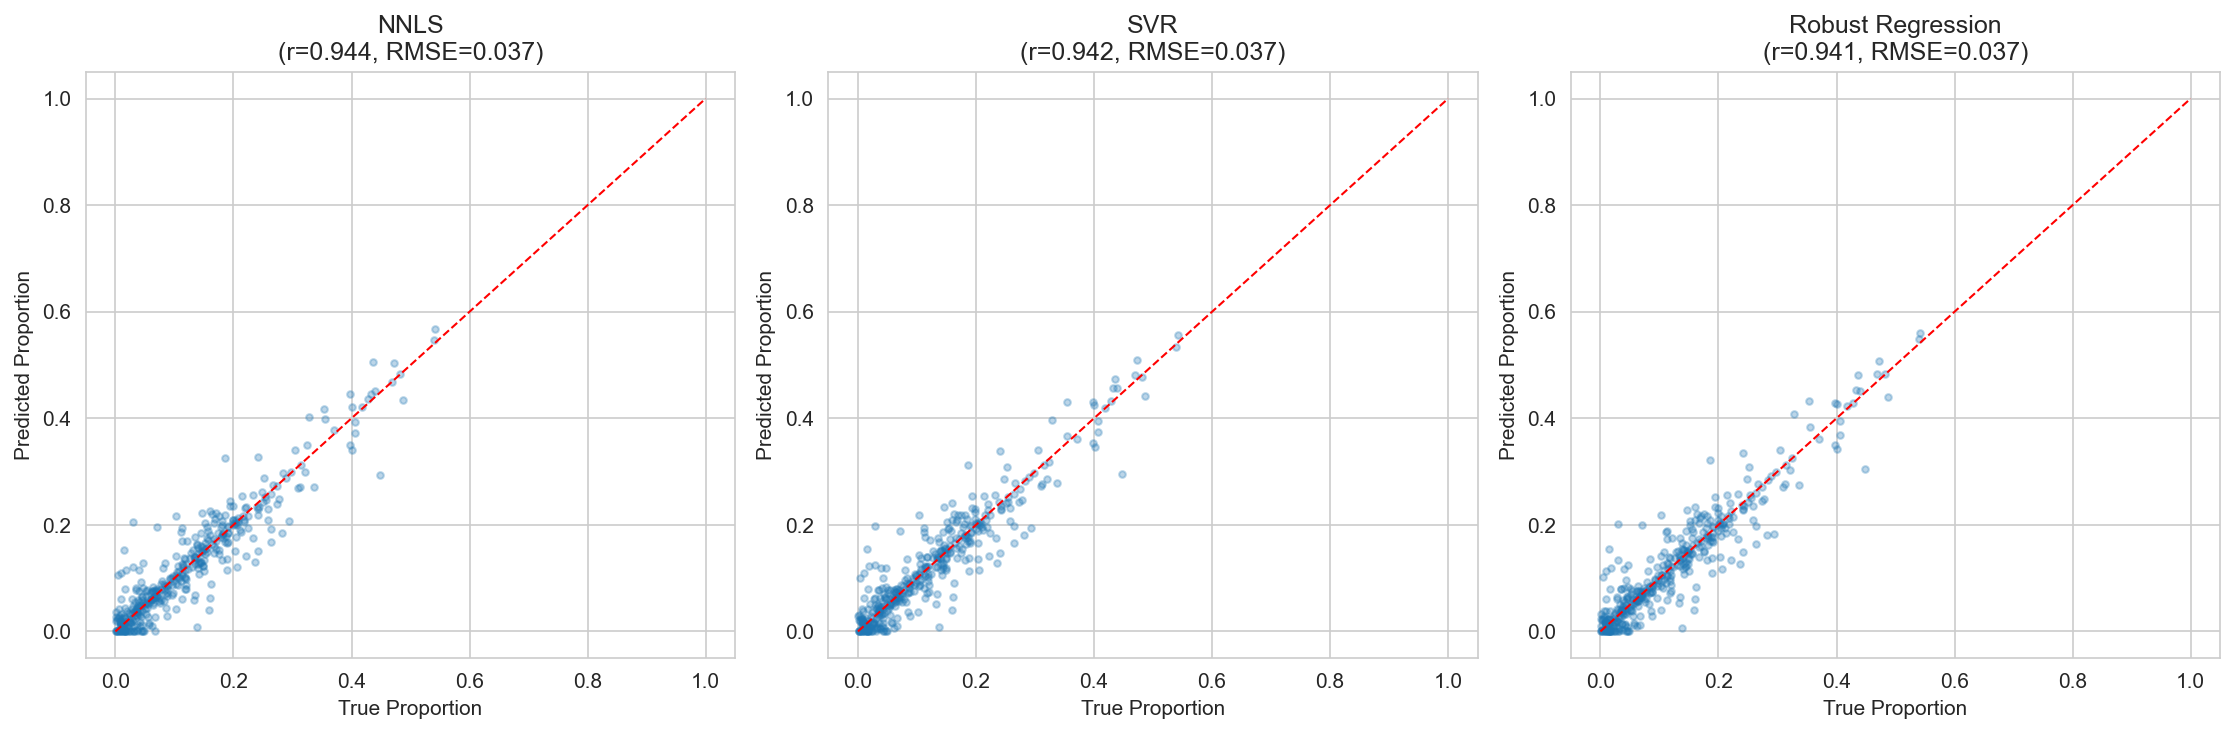
\includegraphics[width=\textwidth]{results/correlation_plots.png}
\caption{True vs.\ predicted cell type proportions for NNLS (\textit{left}),
  SVR (\textit{centre}), and Robust Regression (\textit{right}). The dashed
  line indicates perfect prediction.}
\label{fig:correlation}
\end{figure*}

\subsection{Per-Cell-Type Performance}

Performance varies substantially across cell types (Fig.~\ref{fig:percelltype}).
Basophils, Neutrophils, and Progenitor cells achieve near-perfect accuracy
($r>0.99$), reflecting highly distinctive transcriptomic signatures. T cells
and NK cells are intermediate ($r\approx0.91$--$0.92$), consistent with
shared lymphoid lineage markers. Dendritic cells ($r\approx0.87$) and
Monocytes ($r\approx0.85$) are the hardest to deconvolve due to myeloid
lineage collinearity. This pattern is consistent across all three algorithms.

\begin{figure}[t]
\centering
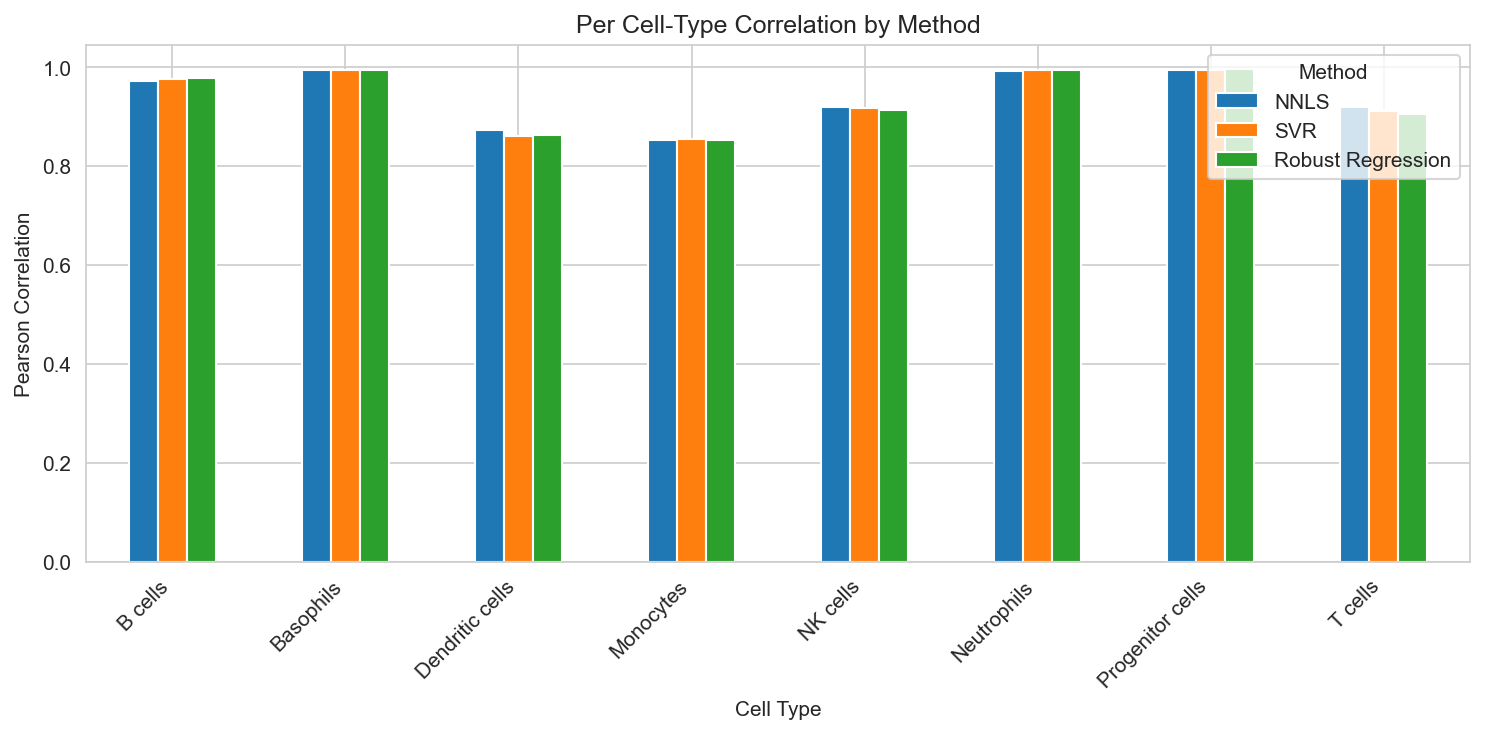
\includegraphics[width=\columnwidth]{results/per_celltype_comparison.png}
\caption{Per-cell-type Pearson $r$ for each method. Myeloid-lineage cells
  show lowest accuracy due to transcriptomic overlap.}
\label{fig:percelltype}
\end{figure}

\subsection{Noise Robustness}

At 100\% noise, Pearson $r$ remains above 0.93 for all methods
(Fig.~\ref{fig:noise}). NNLS is most stable, dropping only 0.0092 across the
full noise range (0.9437 to 0.9345). Robust Regression drops 0.0065, and SVR
degrades the most (0.0103), reaching $r=0.9308$ at maximum noise. The NNLS
non-negativity constraint acts as an implicit regulariser limiting error
accumulation.

\begin{figure}[t]
\centering
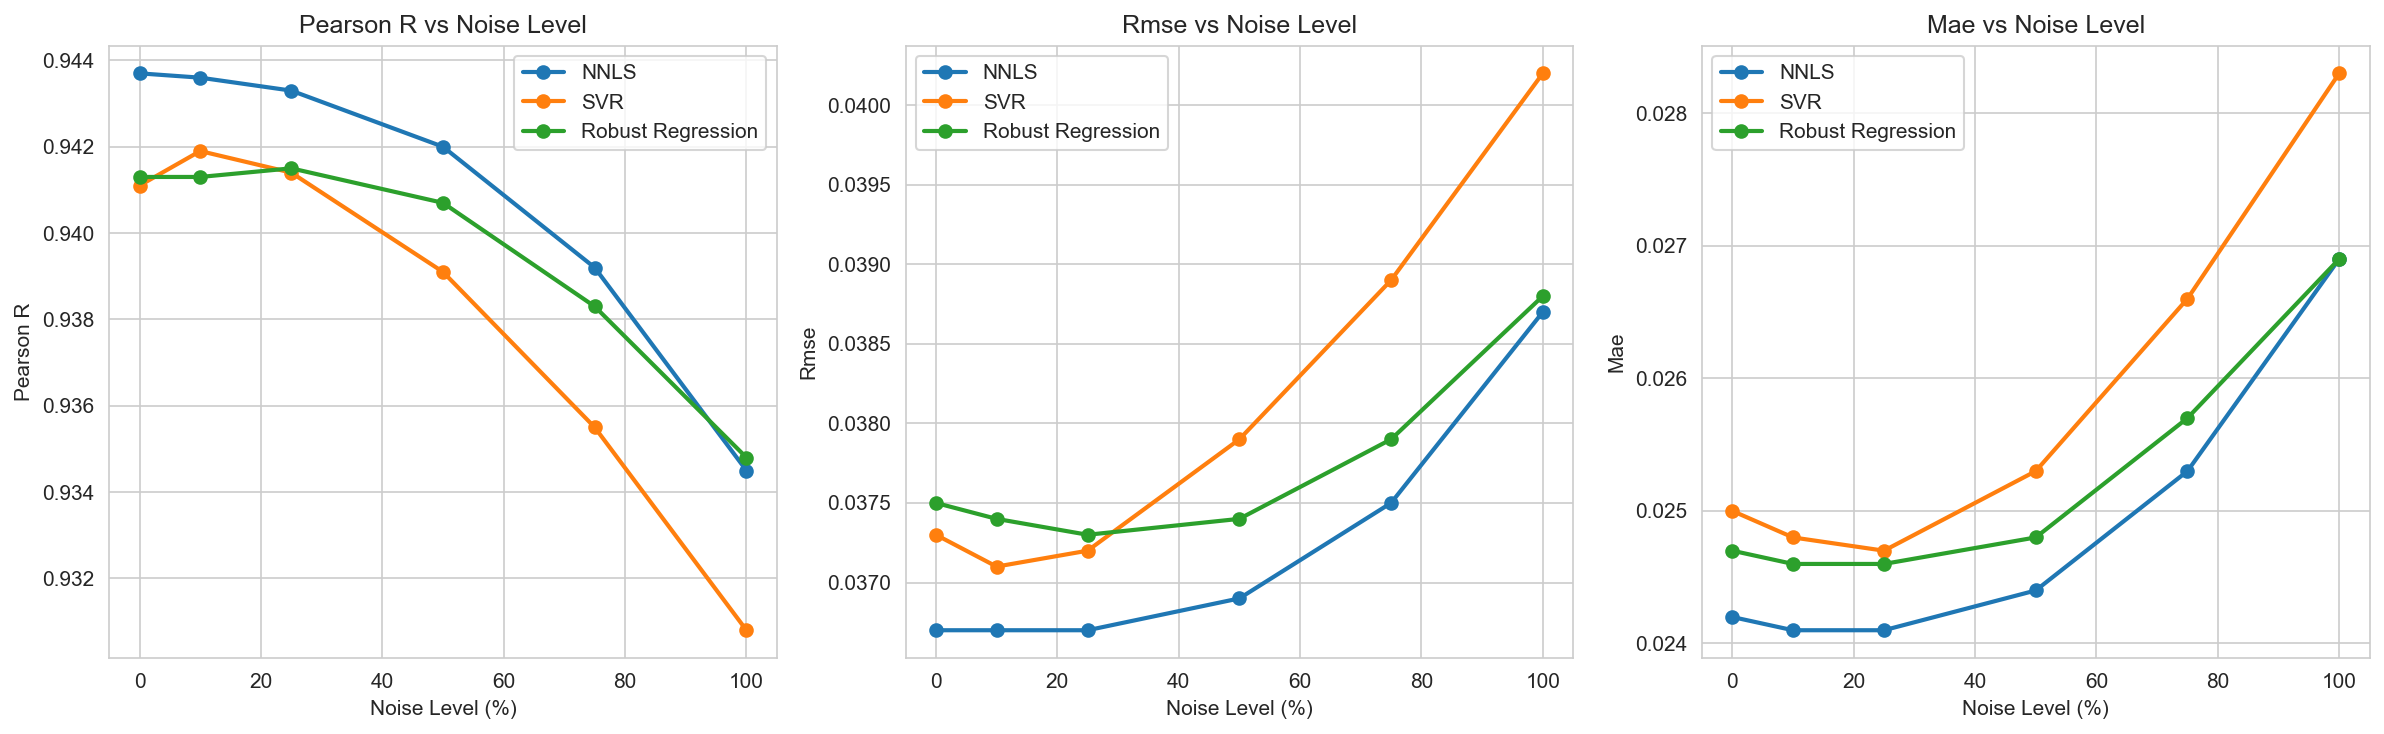
\includegraphics[width=\columnwidth]{results/noise_robustness.png}
\caption{Pearson $r$, RMSE, and MAE vs.\ noise level (0--100\%). NNLS
  maintains the most stable performance.}
\label{fig:noise}
\end{figure}

\subsection{Cell Type Scalability}

A sharp accuracy drop occurs at 4 cell types ($r\approx0.885$;
Fig.~\ref{fig:celltype_var}), corresponding to the simultaneous inclusion
of Monocytes and Dendritic cells, which introduce near-collinearity.
Performance recovers at 5--8 types as each additional transcriptomically
distinct type improves regression conditioning, converging to $r\approx0.94$.

\begin{figure}[t]
\centering
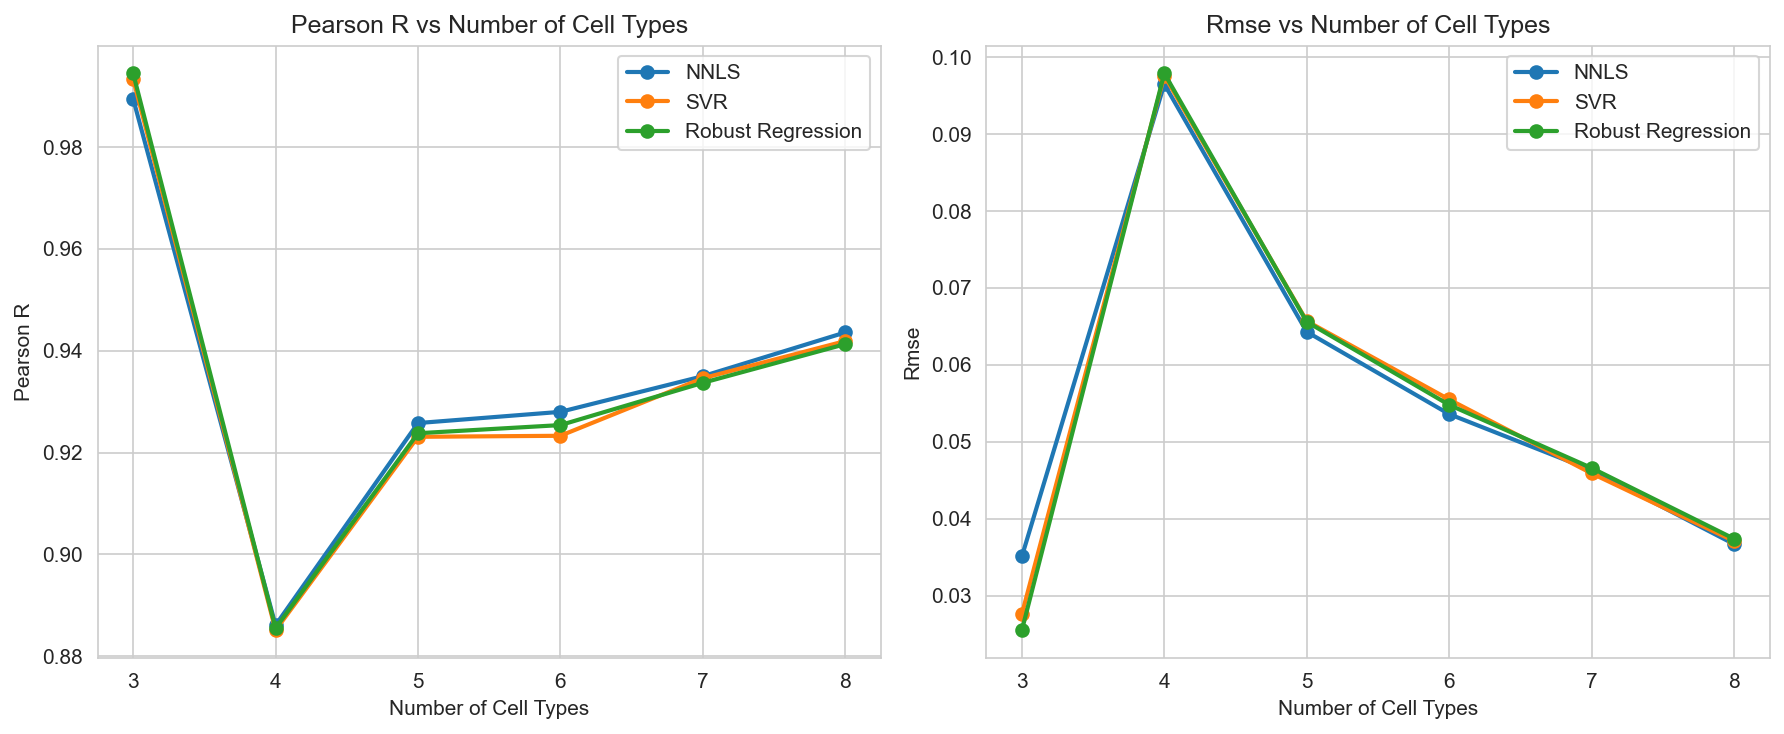
\includegraphics[width=\columnwidth]{results/celltype_variation.png}
\caption{Accuracy and RMSE vs.\ number of deconvolved cell types. The dip
  at 4 cell types reflects signature matrix collinearity.}
\label{fig:celltype_var}
\end{figure}

\subsection{Marker Gene Selection}

At 100 genes, Top Differential Expression achieves $r=0.892$ for NNLS,
outperforming Top Variance ($r=0.853$) and Top Fold Change ($r=0.762$;
Fig.~\ref{fig:markers}). Above 2\,000 genes all strategies converge to
$r\approx0.94$, indicating that selection criterion becomes irrelevant at
sufficient gene coverage.

\begin{figure}[t]
\centering
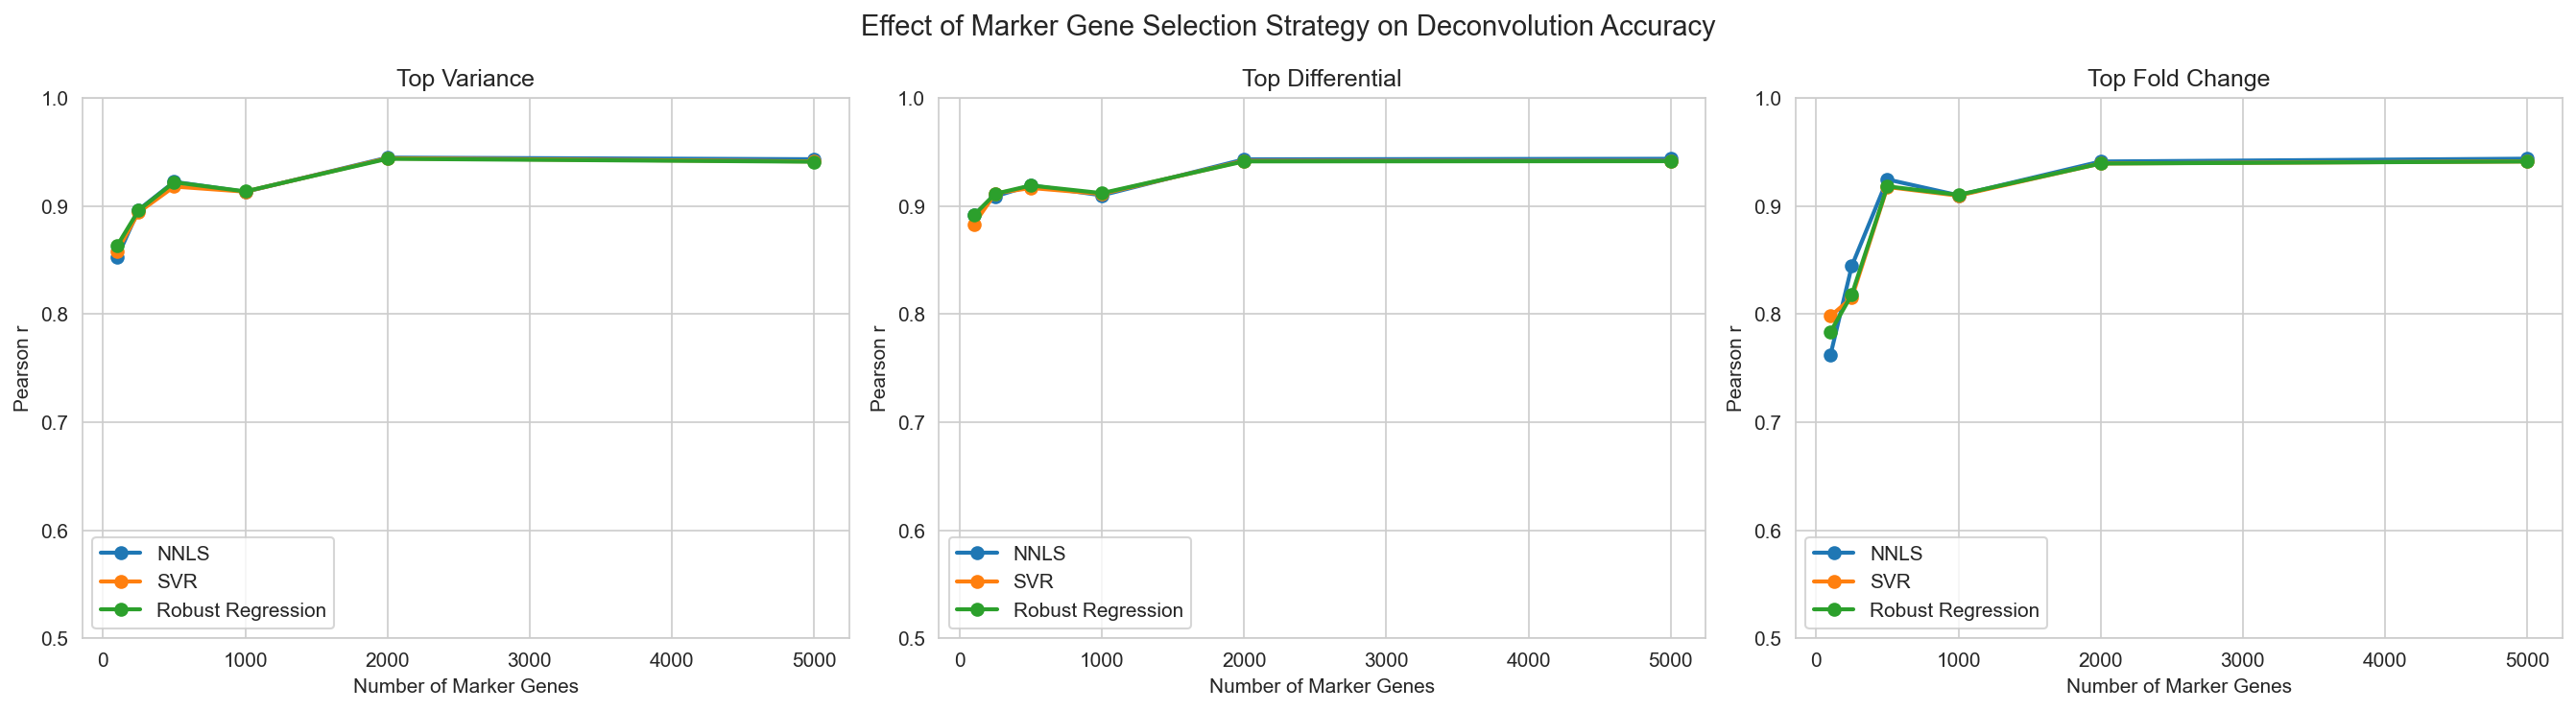
\includegraphics[width=\columnwidth]{results/marker_gene_analysis.png}
\caption{Pearson $r$ vs.\ number of marker genes for three selection
  strategies (NNLS). Top Differential Expression dominates at low gene
  counts.}
\label{fig:markers}
\end{figure}

\subsection{Computational Efficiency}

NNLS (0.04\,s for 50 runs) is 37$\times$ faster than Robust Regression
(1.47\,s) and 2\,970$\times$ faster than SVR (118.8\,s;
Table~\ref{tab:runtime}). Peak memory is comparable across methods
(0.70--1.04\,MB). SVR's runtime scales with support vector count, making it
impractical for high-throughput studies.

\begin{table}[t]
\centering
\caption{Computational cost (50 samples, 8 cell types).}
\label{tab:runtime}
\small
\begin{tabular}{lcc}
\toprule
Method & Runtime (s) & Peak Memory (MB) \\
\midrule
NNLS         & 0.04   & 1.04 \\
Robust Regr. & 1.47   & 0.73 \\
SVR          & 118.80 & 0.70 \\
\bottomrule
\end{tabular}
\end{table}

% ================================================================
\section{Discussion}

Three algorithms with fundamentally different mathematical formulations
produce nearly identical deconvolution accuracy ($\Delta r<0.003$), strongly
suggesting the regression engine is not a meaningful axis of variation at
sufficient gene coverage. We recommend NNLS for production pipelines: it
matches or exceeds competitors on accuracy, is most noise-stable, and is
nearly three orders of magnitude faster than SVR. Its simplicity---single
convex optimisation, no hyperparameters---also makes it easy to audit and
reproduce.

The primary accuracy determinant is not the regression algorithm but the
reference signature matrix structure. The Monocyte/Dendritic cell accuracy
floor ($r\approx0.85$--$0.87$) is consistent across all methods and reflects
biological reality: myeloid cells share transcriptional programmes creating
irreducible collinearity. Future work should explore condition-number-aware
regularisation, hierarchical deconvolution strategies (lineage separation
before sub-deconvolution), or lineage-specific marker panels. Marker gene
selection is the second most important factor: Top Differential Expression
consistently outperforms alternatives when gene budgets are constrained.

\paragraph{Limitations.}
Synthetic pseudo-bulk mixtures assume linear mixing; real tissue may include
cell--cell interactions and spatial heterogeneity not captured here. We tested
only 8 cell types; real atlases with 20 or more may amplify collinearity
effects. All experiments used a single reference dataset, leaving
cross-platform generalisation to future work. Deep learning deconvolution
approaches such as Scaden \citep{menden2020} may handle collinear cell types
more gracefully and represent a promising direction for future comparison.

% ================================================================
\section{Conclusion}

We benchmarked NNLS, SVR, and Robust Regression for reference-based bulk
RNA-seq deconvolution across accuracy, noise robustness, scalability, and
marker gene sensitivity. NNLS achieves the best overall trade-off: highest
accuracy ($r=0.9436$), greatest noise stability, and $\approx$3\,000$\times$
faster execution than SVR. Marker gene selection strategy and cell type
transcriptomic distinctness are the dominant determinants of quality.
These findings provide actionable guidance: invest effort in signature matrix
quality and gene selection rather than in complex regression formulations.

% ================================================================
\section*{Funding}

Completed as a course project for CS\,502 at the University of Illinois
Chicago. No external funding received.

% ================================================================
\bibliographystyle{plainnat}
\begin{thebibliography}{7}

\bibitem[Newman \textit{et~al}.(2019)]{newman2019}
Newman,~A.M., Steen,~C.B., Liu,~C.L., Gentles,~A.J., Chaudhuri,~A.A.,
Scherer,~F.\ \textit{et~al}.\ (2019).
Determining cell type abundance and expression from bulk tissues with digital
cytometry.
\textit{Nature Biotechnology}, \textbf{37}(7):773--782.

\bibitem[Wang \textit{et~al}.(2019)]{wang2019}
Wang,~X., Park,~J., Susztak,~K., Zhang,~N.R., and Li,~M.\ (2019).
Bulk tissue cell type deconvolution with multi-subject single-cell expression
reference.
\textit{Nature Communications}, \textbf{10}(1):380.

\bibitem[Avila~Cobos \textit{et~al}.(2020)]{avilacobo2020}
Avila~Cobos,~F., Vandesompele,~J., Mestdagh,~P., and De~Preter,~K.\ (2020).
Computational deconvolution of transcriptomics data from mixed cell
populations.
\textit{Bioinformatics}, \textbf{36}(5):1517--1527.

\bibitem[Sturm \textit{et~al}.(2019)]{sturm2019}
Sturm,~G., Finotello,~F., Petitprez,~F., Zhang,~J.D., Baumbach,~J.,
Fridman,~W.H.\ \textit{et~al}.\ (2019).
Comprehensive evaluation of transcriptome-based cell-type quantification
methods for immuno-oncology.
\textit{Bioinformatics}, \textbf{35}(14):i436--i445.

\bibitem[Racle \textit{et~al}.(2017)]{racle2017}
Racle,~J., de~Jonge,~K., Baumgaertner,~P., Speiser,~D.E., and
Gfeller,~D.\ (2017).
Simultaneous enumeration of cancer and immune cell types from bulk tumor
gene expression data.
\textit{eLife}, \textbf{6}:e26476.

\bibitem[Finotello \textit{et~al}.(2019)]{finotello2019}
Finotello,~F., Mayer,~C., Plattner,~C., Laschober,~G., Rieder,~D.,
Hackl,~H.\ \textit{et~al}.\ (2019).
Molecular and pharmacological modulators of the tumor immune contexture
revealed by deconvolution of RNA-seq data.
\textit{Genome Medicine}, \textbf{11}(1):34.

\bibitem[Menden \textit{et~al}.(2020)]{menden2020}
Menden,~K., Marouf,~M., Oller,~S., Dalmia,~A., Kloiber,~K., Heutink,~P.,
and Bonn,~S.\ (2020).
Deep learning-based cell composition analysis from tissue expression profiles.
\textit{Science Advances}, \textbf{6}(30):eaba2619.

\end{thebibliography}

\end{document}
